\section*{Introduction}

Skin cancer, including melanoma, is a significant global public health concern.
Melanoma presents a considerable challenge due to its high mortality rate and
the critical importance of early detection for successful treatment. Cancer
begins when healthy cells undergo changes that cause them to grow and divide
uncontrollably, forming tumors. These tumors can be classified as either
cancerous (malignant) or non-cancerous (benign).\\

In recent times, there has been a growing focus on automating tasks in the
medical field through Computer-Aided Diagnosis (CAD)\footnote{CAD refers to the
use of computer algorithms and technologies to assist healthcare professionals
in the process of medical diagnosis.}. Some studies have demonstrated that
these systems can achieve results similar to those of professionals. However,
the integration of CAD into the medical system remains a significant challenge. \\

Firstly, certain methods are constructed based on theoretical models of
melanoma appearance, which may restrict their applicability to specific
morphologies and fail to capture the wide range of variations seen in
real-world scenarios. Secondly, the artificial intelligence (AI) systems
utilized in these classifiers are trained to address singular and narrow tasks.
Unlike human dermatologists, these systems lack the ability to consider
holistic patient information when formulating a final diagnosis, reflecting the
concept of weak AI \cite{WeakAI}. Lastly, numerous methods have been trained
and evaluated using high-quality image frames, which may result in instability
when applied under real-time conditions where image quality is often
compromised. \\

Overcoming these constraints and creating melanoma cancer classifiers that
encompass an extended array of morphologies, integrate comprehensive patient
information, and exhibit resilience in real-world situations are essential
steps in the development of automated tools that can provide assistance to
healthcare professionals.

\newpage

\section*{Objectives}

The main objective of this thesis is to create a health care infrastructure,
focused on melanoma detection using deep learning methods to train a system
capable of detecting melanoma on dermoscopy images to test the ability of
computer-assisted image analysis. To this end, the gradual achievements that
must be accomplished are:

\begin{itemize}

  \item Gaining a comprehensive understanding of the theory
    behind deep learning and its practical applications.

  \item Explore and study the optimal approach for utilizing the distribution
    of dermoscopy images from the dataset during the training process.

  \item Propose and train deep learning models with different techniques based on
    tranfer-learning, exploiting images of the melanoma
    ISIC\footnote{International Skin Imaging Collaboration. An international
    effort to improve melanoma diagnosis.} Challenge \cite{IsicChallenge}.

  \item Developing a CAD infrastructure. The CAD infrastructure, should contain
    the already trained models with a simple web UI\footnote{User Interface. Is
    the point of human-computer interaction and communication in a device.}an
    API\footnote{Application Programming Interface. Is a set of protocols,
      routines, tools, and definitions that allow different software applications
    to communicate with each othe} and finally a mechanism using Docker to create
    the images of the services making it ease to deploy in any based Linux System.

\end{itemize}


\section*{Development Process}

The project methodology employed in this endeavor follows a continuous process
that builds upon previous approaches. Additionally, the project incorporates
the concept of utilizing idle time effectively. For instance, during the
training of models, there are periods of idle time, which we exploited by
concurrently working on other tasks related to developing the entire
infrastructure. This approach allows for maximizing productivity throughout the
project (see Figure \ref{fig:flux_development}).

\newpage

\begin{landscape}

  \begin{figure}[H]
  \centering
  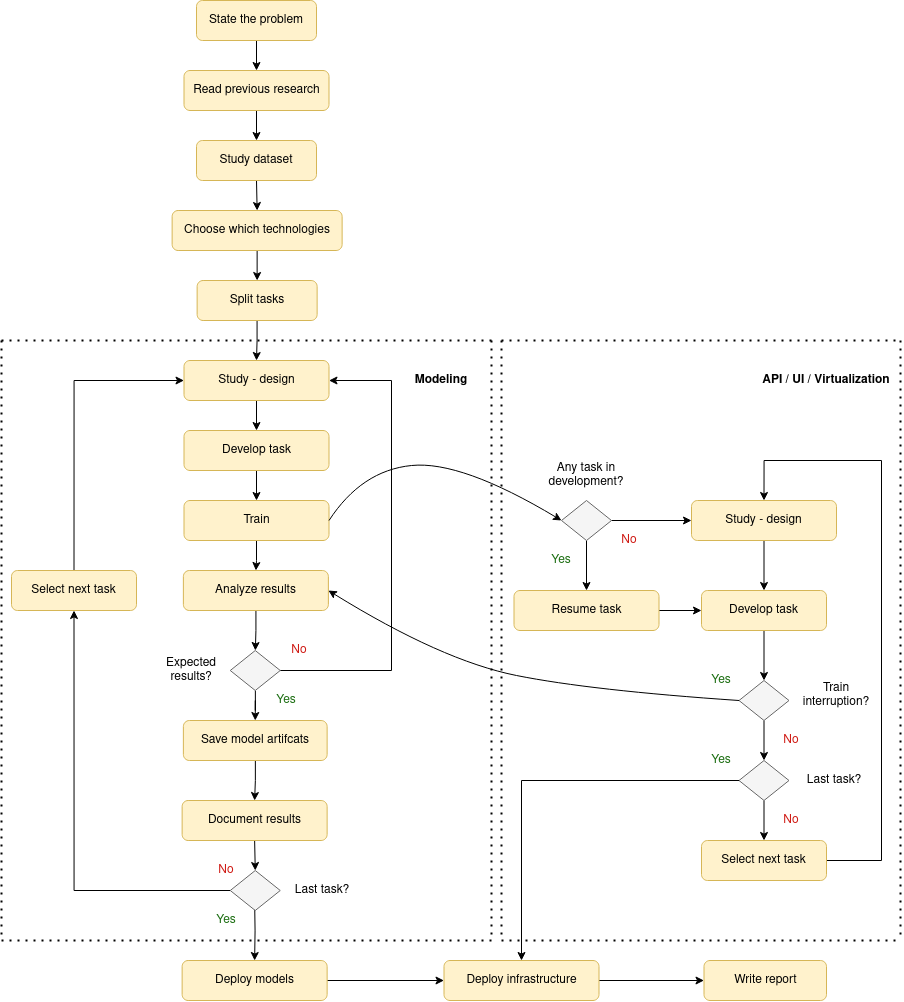
\includegraphics[width=0.82\textwidth]{imatges/planing_and_methodology/EmplyedMethodology.png}
  \caption{Activity diagram describing the methodology.}
  \label{fig:flux_development}
  \end{figure}

\end{landscape}


The process used to train, validate, test, and implement the models is
illustrated in Figure \ref{fig:cad-infrastructure-training-system}. This
sequence consists of several stages elaborated below. \\

The first stage involves cleaning and splitting the initial dataset into
smaller datasets. This step ensures that the data is organized and ready for
further processing. \\

The second stage focuses on training and validating the models using the
training and validation datasets. During this stage, the system reads images
and applies data augmentation techniques to train images and Test Time
Augmentation (TTA) to validation images. These techniques enhance the model's
performance by introducing variations in the data and improving its
generalization ability. \\

The third stage involves analyzing the training results obtained from different
training approaches. In this section*, we evaluate and analyze the model's
performance by comparing the predicted results against the test dataset. This
step helps us understand how well the models are learning and performing on
unseen data. \\

The last stage revolves around exposing the trained models through an API's
container image. This container image allows for easy deployment and
integration of the models into other systems or applications, providing a
convenient way to utilize the trained models for various tasks. \\


\begin{figure}[H]
  %\begin{adjustbox}{width=\textwidth, trim={0.2cm 0pt 1.5cm 0pt}, clip}
  \centering
  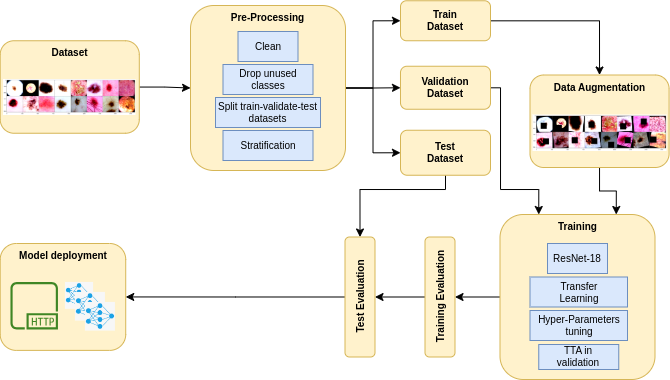
\includegraphics[width=0.9\textwidth]{imatges/methodological_contribution/Pipeline.drawio.png}
  %\end{adjustbox}
  \caption[CAD infrastructure pipeline]{\textit{CAD infrastructure pipeline. }}
  {\label{fig:cad-infrastructure-training-system}}
\end{figure}

\section*{Results}

The training phase ended with the development of eight models using an
imbalanced dataset comprising eight classes. Various learning policies and
Artificial Intelligence (AI) techniques were tested during the experimentation
process.  \\

These models were divided into two categories: one without any
additional regularization and another with additional regularization techniques
such as data augmentation and the inclusion of dropout layers.

\begin{table}[H]
\centering
\begin{tabular}{lc|lc}
    \toprule
  \textbf{Model} & \textbf{Test AUC} & \cellcolor{gray!50}\textbf{Model} & \cellcolor{gray!50}\textbf{Test AUC}  \\
\midrule
 M0 & 0.892 & \cellcolor{gray!50}M4 & \cellcolor{gray!50}0.858 \\
 M1 $\star$ & 0.892 & \cellcolor{gray!50}M5 $\star$ & \cellcolor{gray!50}0.843 \\
 M2 $\ast$ &  0.885 &  \cellcolor{gray!50}M6 $\ast$ & \cellcolor{gray!50}0.848 \\
 M3 $\bullet$ & 0.886 & \cellcolor{gray!50}M7 $\bullet$ & \cellcolor{gray!50}0.849 \\
 \midrule
Mean &  88.875\% & \cellcolor{gray!50}Mean & \cellcolor{gray!50}84.950\%  \\
SD &  0.377\%  &   \cellcolor{gray!50}SD &  \cellcolor{gray!50}0.625\%  \\

\bottomrule
\end{tabular}
\caption[Models metrics in test dataset]
  {\textit{Models metrics in test dataset.}}
{\label{table:test-set-resume-metrics}}
\end{table}

The initial group of models, lacking extra regularization, displayed impressive
performance on the test set, boasting a mean AUC metric of 88.875\% with a minor
standard deviation of ±0.377\%. However, this group exhibited signs of
overfitting during training, as evidenced by their performance on the
validation set. In contrast, the second group of models, which underwent
training with additional regularization techniques, achieved lower results
compared to the first group. Nonetheless, these models did not suffer from
overfitting, indicating potential for improved results with extended training
epochs. The second group of models attained an average AUC of 84.950\% with a
standard deviation of ±0.625\%. The increase in standard deviation in the second
group is attributed to the impact of using more training epochs, rendering the
behavior of the schedulers more noticeable. \\

Concurrently, while in the model training phase, we seized the opportunity to
build the CAD infrastructure required to support the project. For
the API, we embraced a flexible approach utilizing soft configurations,
allowing for the specification of settings through file-based parameters. This
approach offers both adaptability and simplified management. Furthermore, we
meticulously crafted an intuitive and UI to
facilitate seamless interaction between healthcare professionals and the
accessible models (refer to Figures \ref{fig:ui-tools} to \ref{fig:extra-inf-popup}). \\

Moreover, we have included a script to initiate the infrastructure, leveraging
Docker images, which can be executed on any Linux operating system. This script
ensures the efficient startup of the infrastructure components, enhancing the
ease of deployment and operation.

\begin{figure}[H]
  \centering
  \begin{adjustbox}{width=\textwidth, trim={0.2cm 0cm 0.1cm 0cm}, clip}
    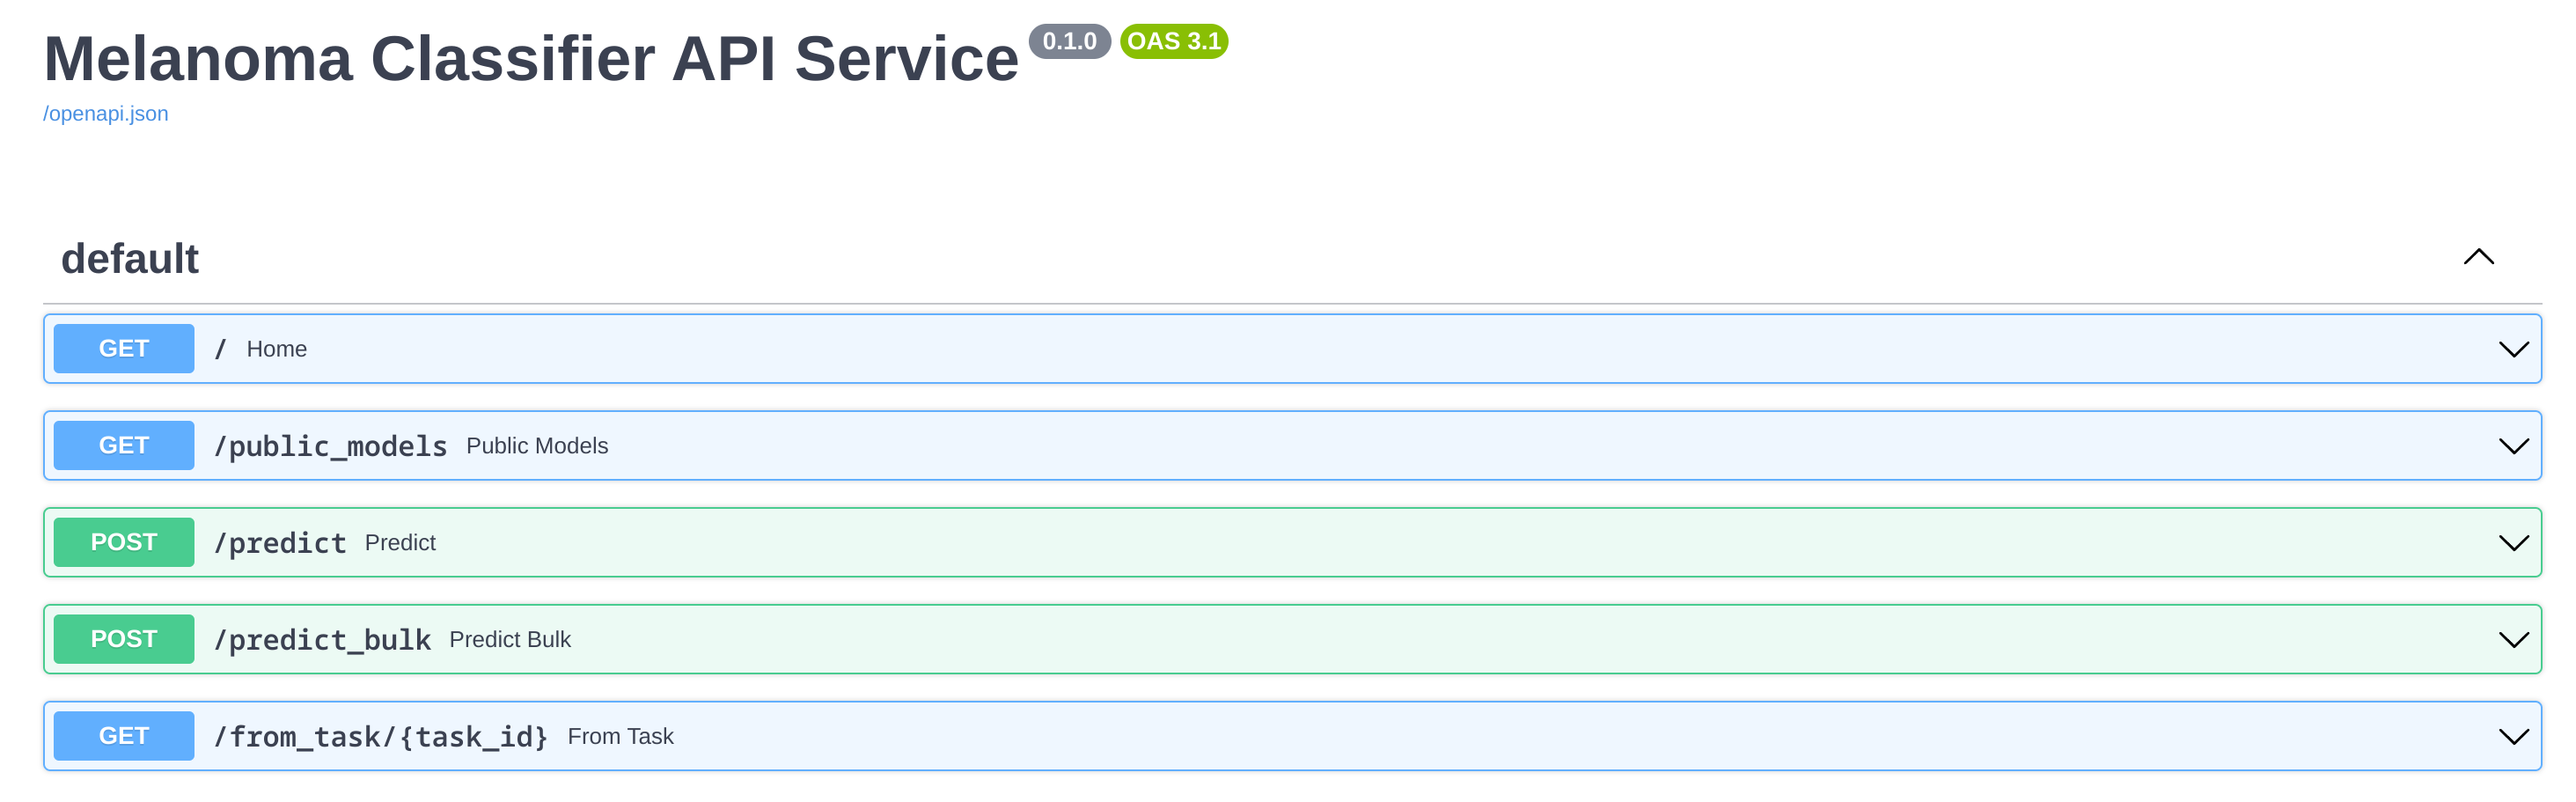
\includegraphics[width=\textwidth]{imatges/results/api-endpoints.png}
  \end{adjustbox}
  \caption[API service End-Points]{\textit{API service End-Points. }}
  {\label{fig:api-endpoints}}
\end{figure}

\begin{figure}[H]
  \centering
  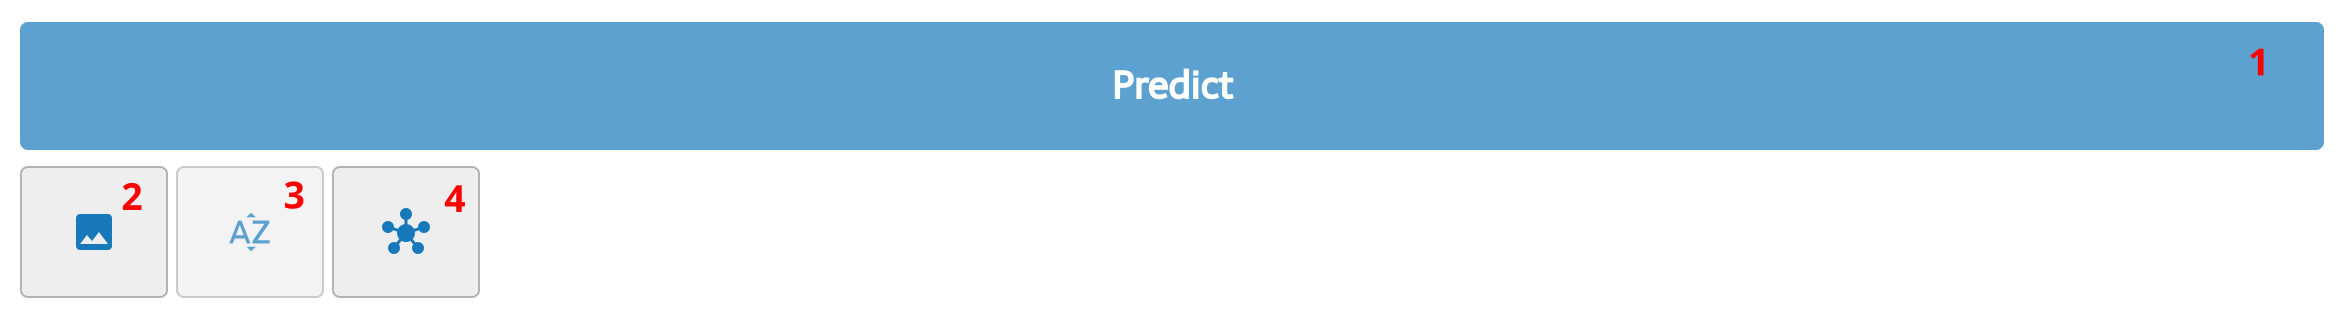
\includegraphics[width=\textwidth]{imatges/results/ui-tools.png}
  \caption[Main interactive Buttons of the UI service]{\textit{Main interactive buttons of the UI service. }}
  {\label{fig:ui-tools}}
\end{figure}

\begin{figure}[H]
  \centering
  \begin{adjustbox}{width=\textwidth, trim={0.05cm 1.25cm 0cm 0.1cm}, clip}
    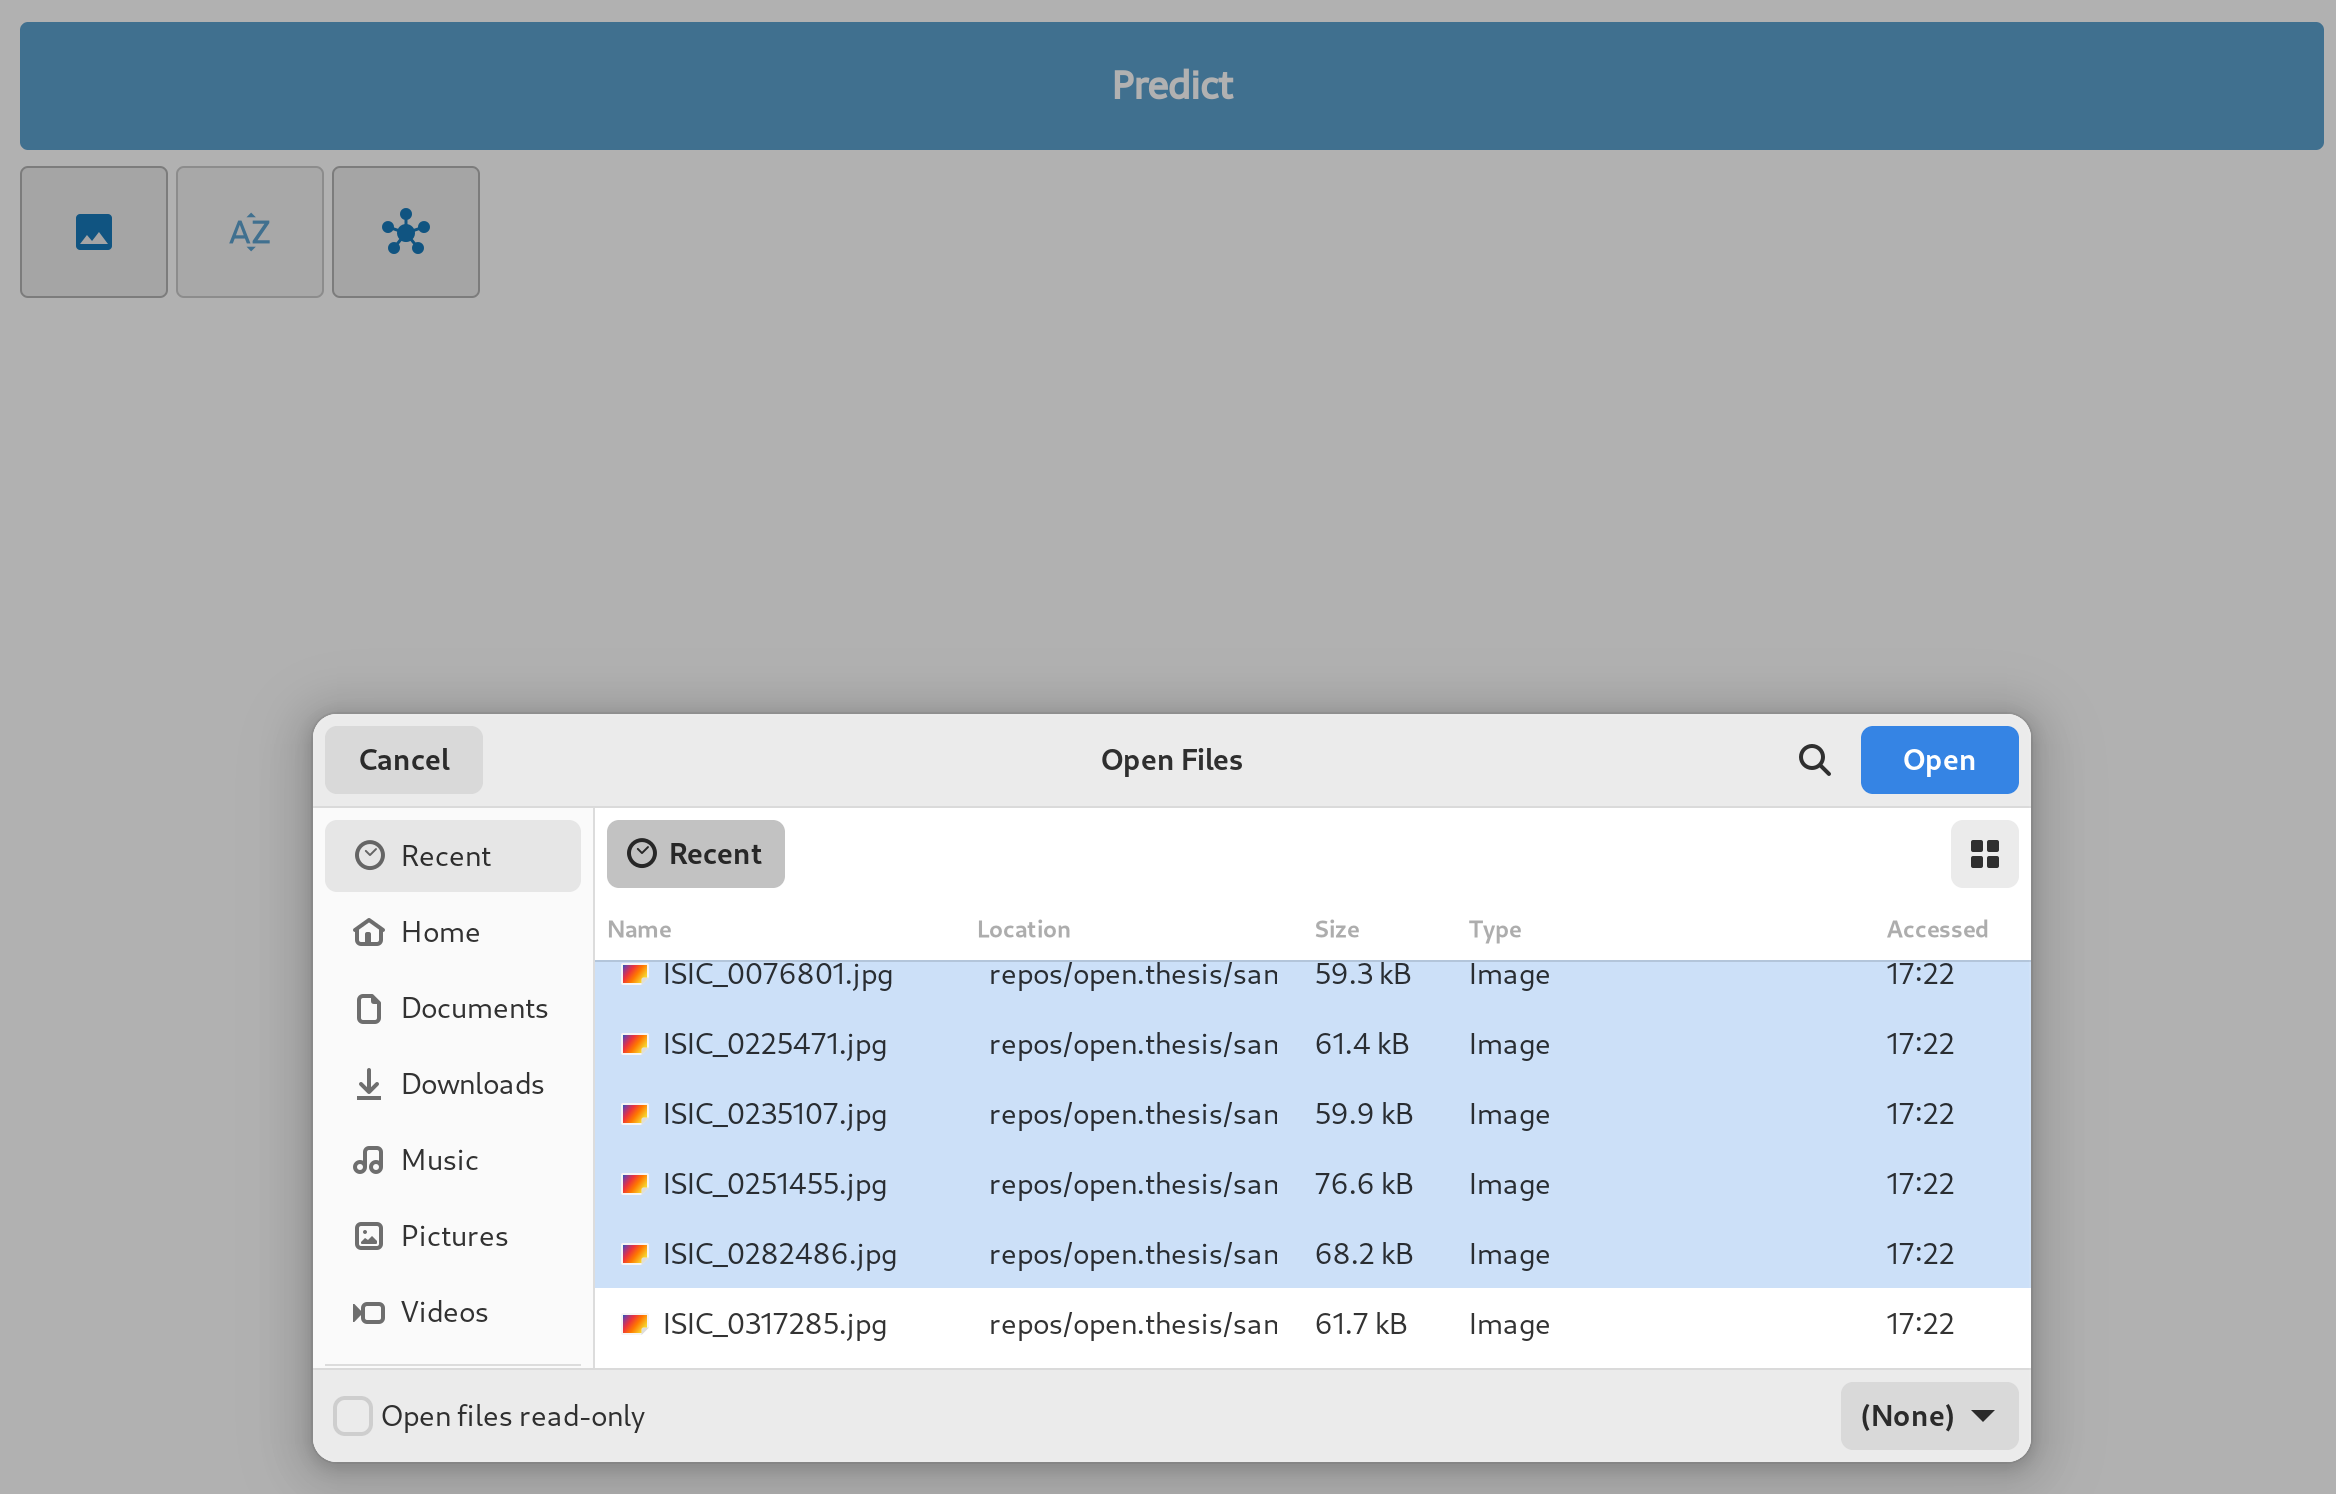
\includegraphics[width=\textwidth]{imatges/results/selecting-images.png}
  \end{adjustbox}
  \caption[Loading dermoscopy images from device]{\textit{Loading dermoscopy images from device. }}
  {\label{fig:selecting-imgs}}
\end{figure}

\begin{figure}[H]
  \centering
  \begin{adjustbox}{width=\textwidth, trim={0cm 3.5cm 0cm 0cm}, clip}
    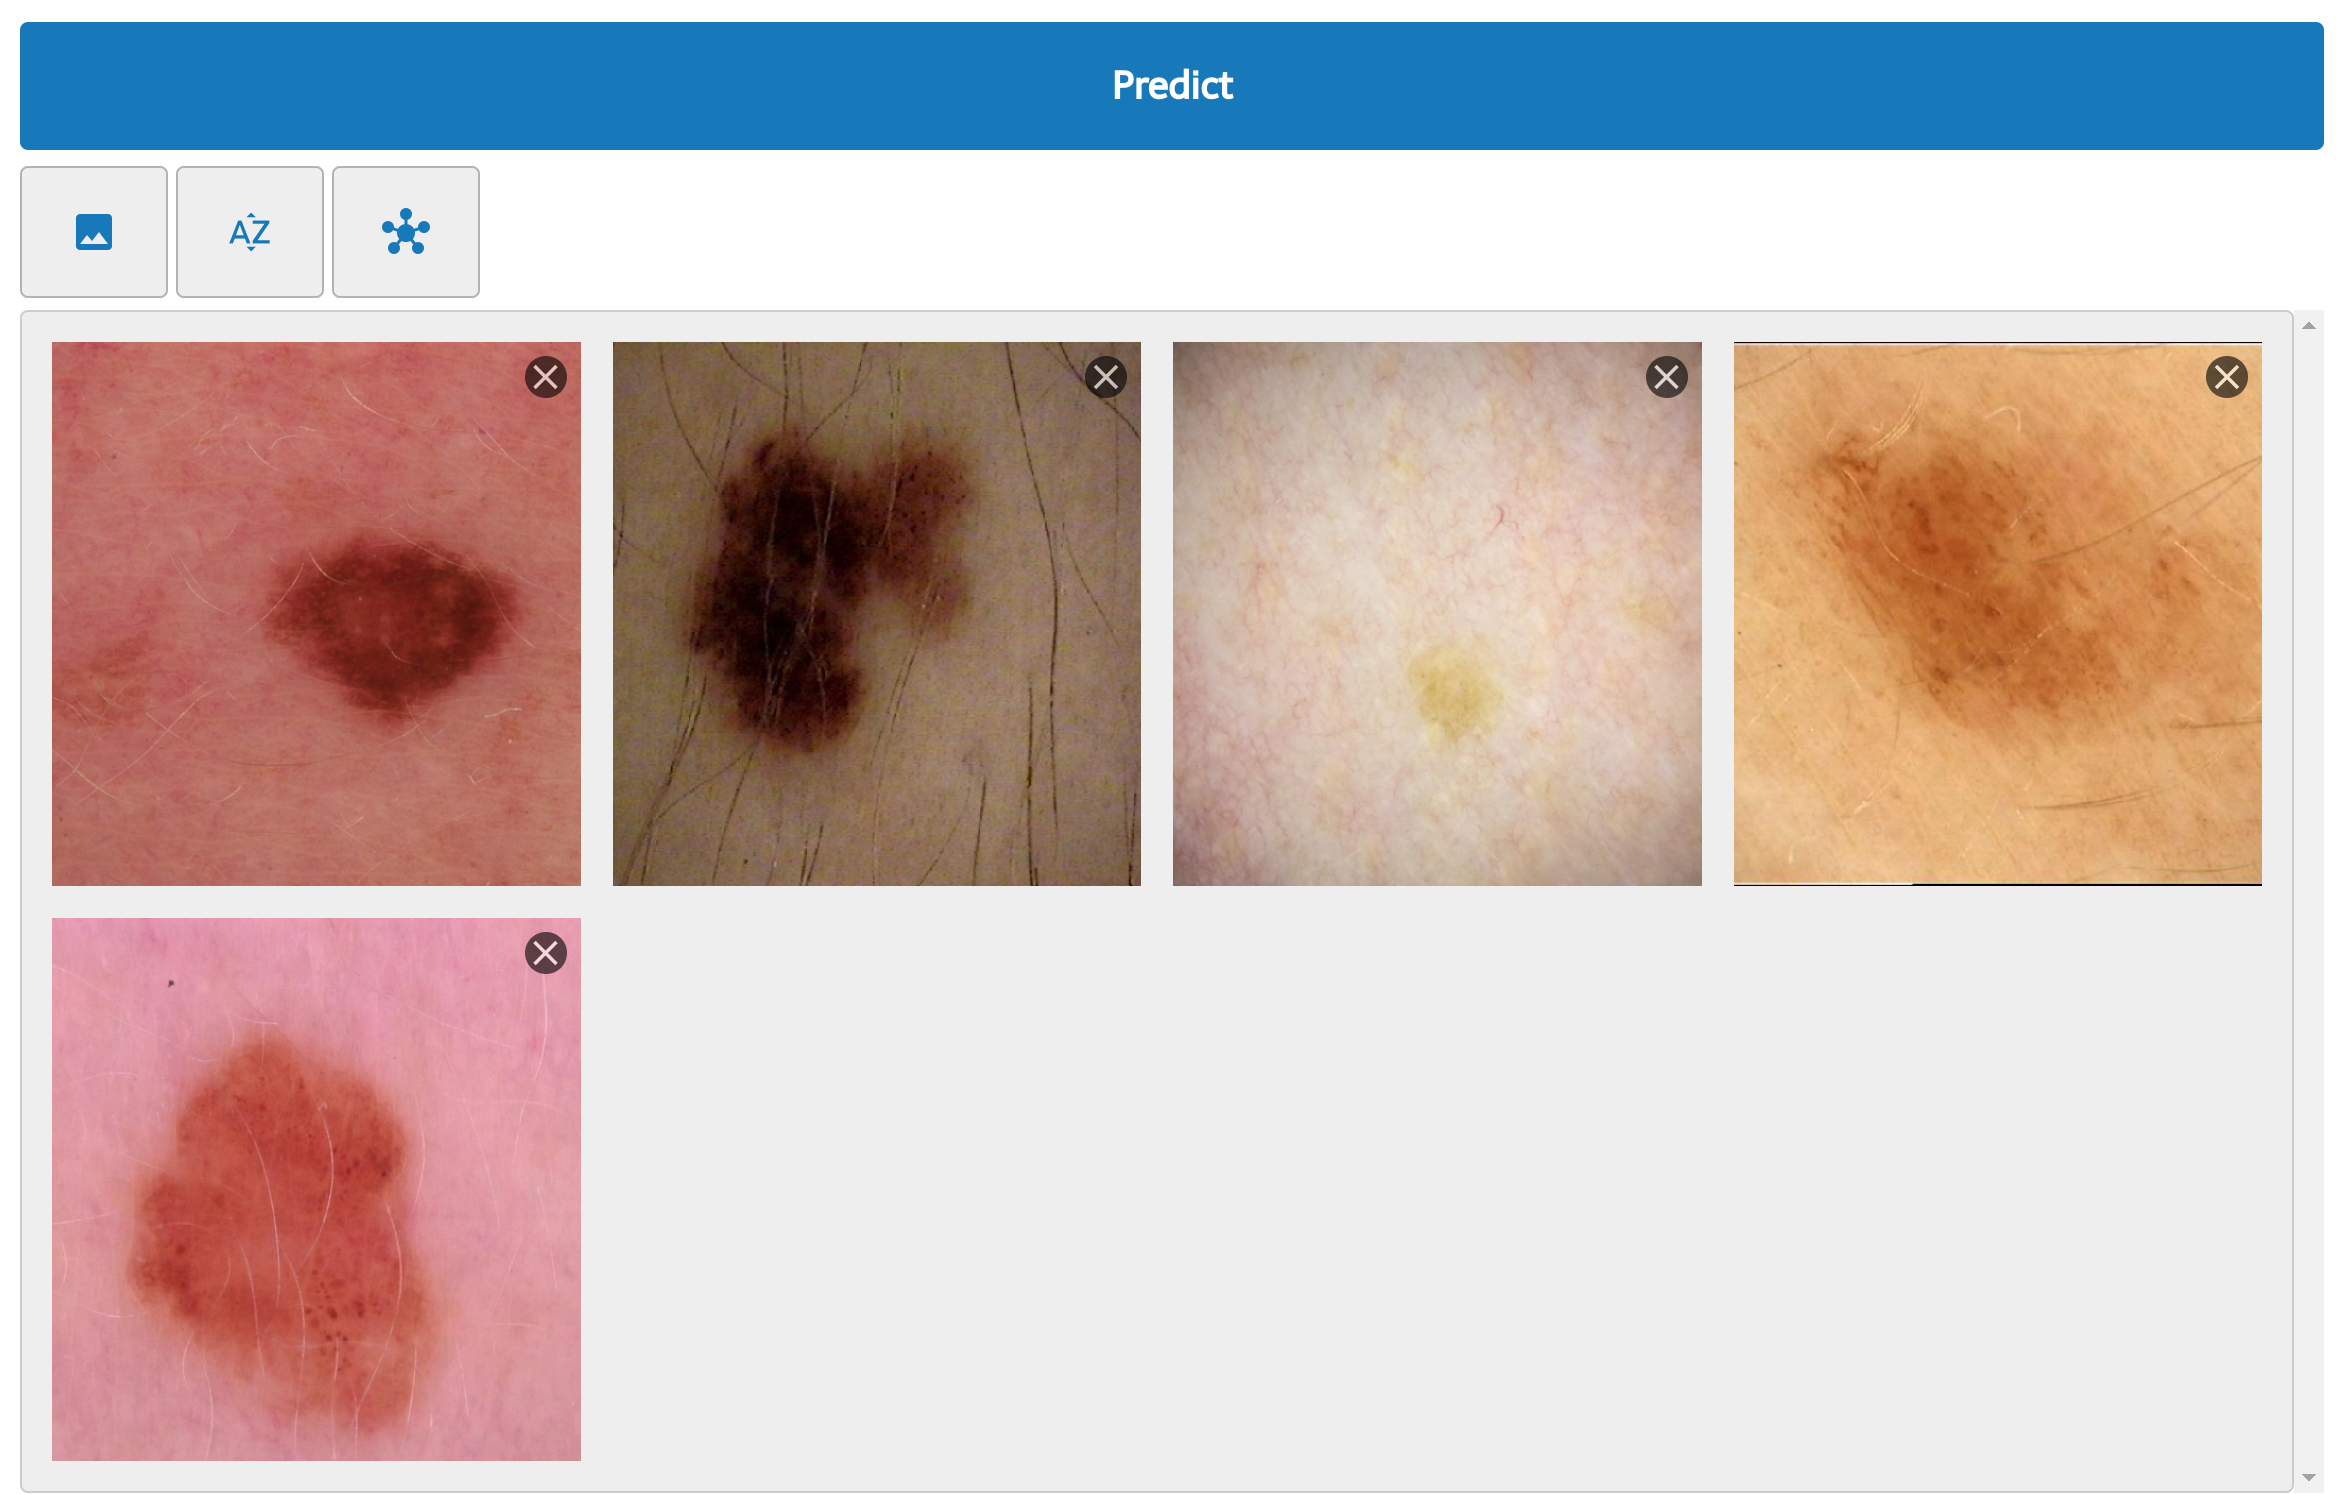
\includegraphics[width=\textwidth]{imatges/results/loaded-images.png}
  \end{adjustbox}
  \caption[Dermoscopy images loaded in the UI]{\textit{Dermoscopy images loaded in the UI. }}
  {\label{fig:loaded-images}}
\end{figure}

\begin{figure}[H]
  \centering
  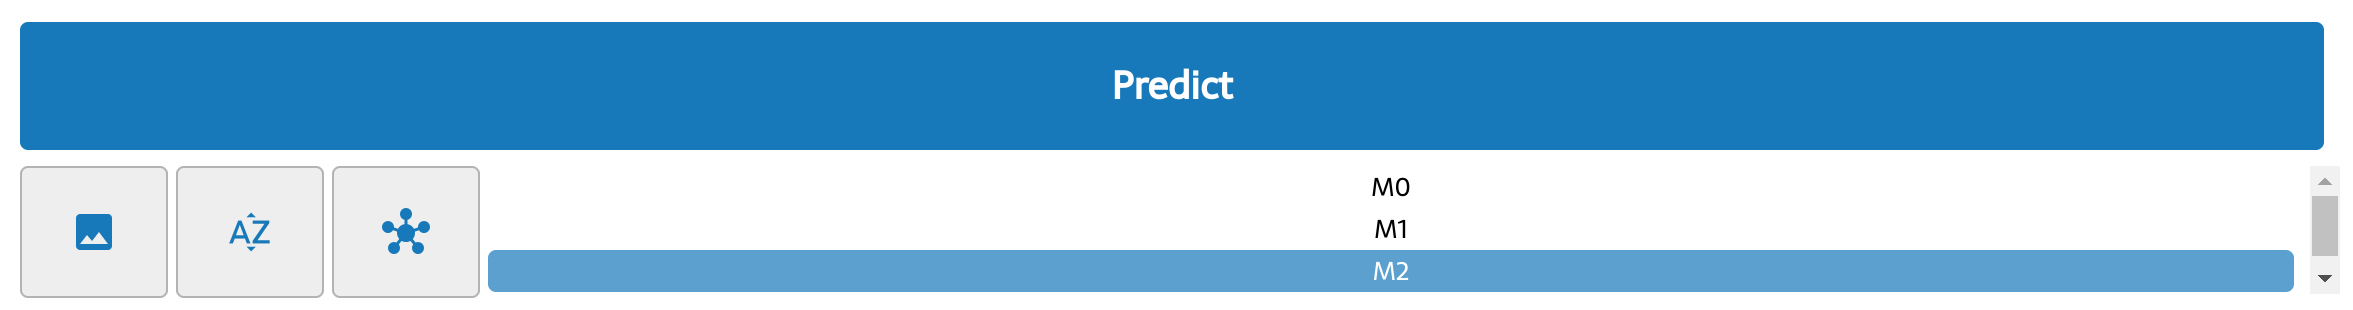
\includegraphics[width=\textwidth]{imatges/results/selecting-model.png}
  \caption[Selecting exposed models by the API]{\textit{Selecting exposed models by the API. }}
  {\label{fig:selecting-model}}
\end{figure}

\begin{figure}[H]
  \centering
  \begin{adjustbox}{width=\textwidth, trim={0cm 3.55cm 0cm 0cm}, clip}
    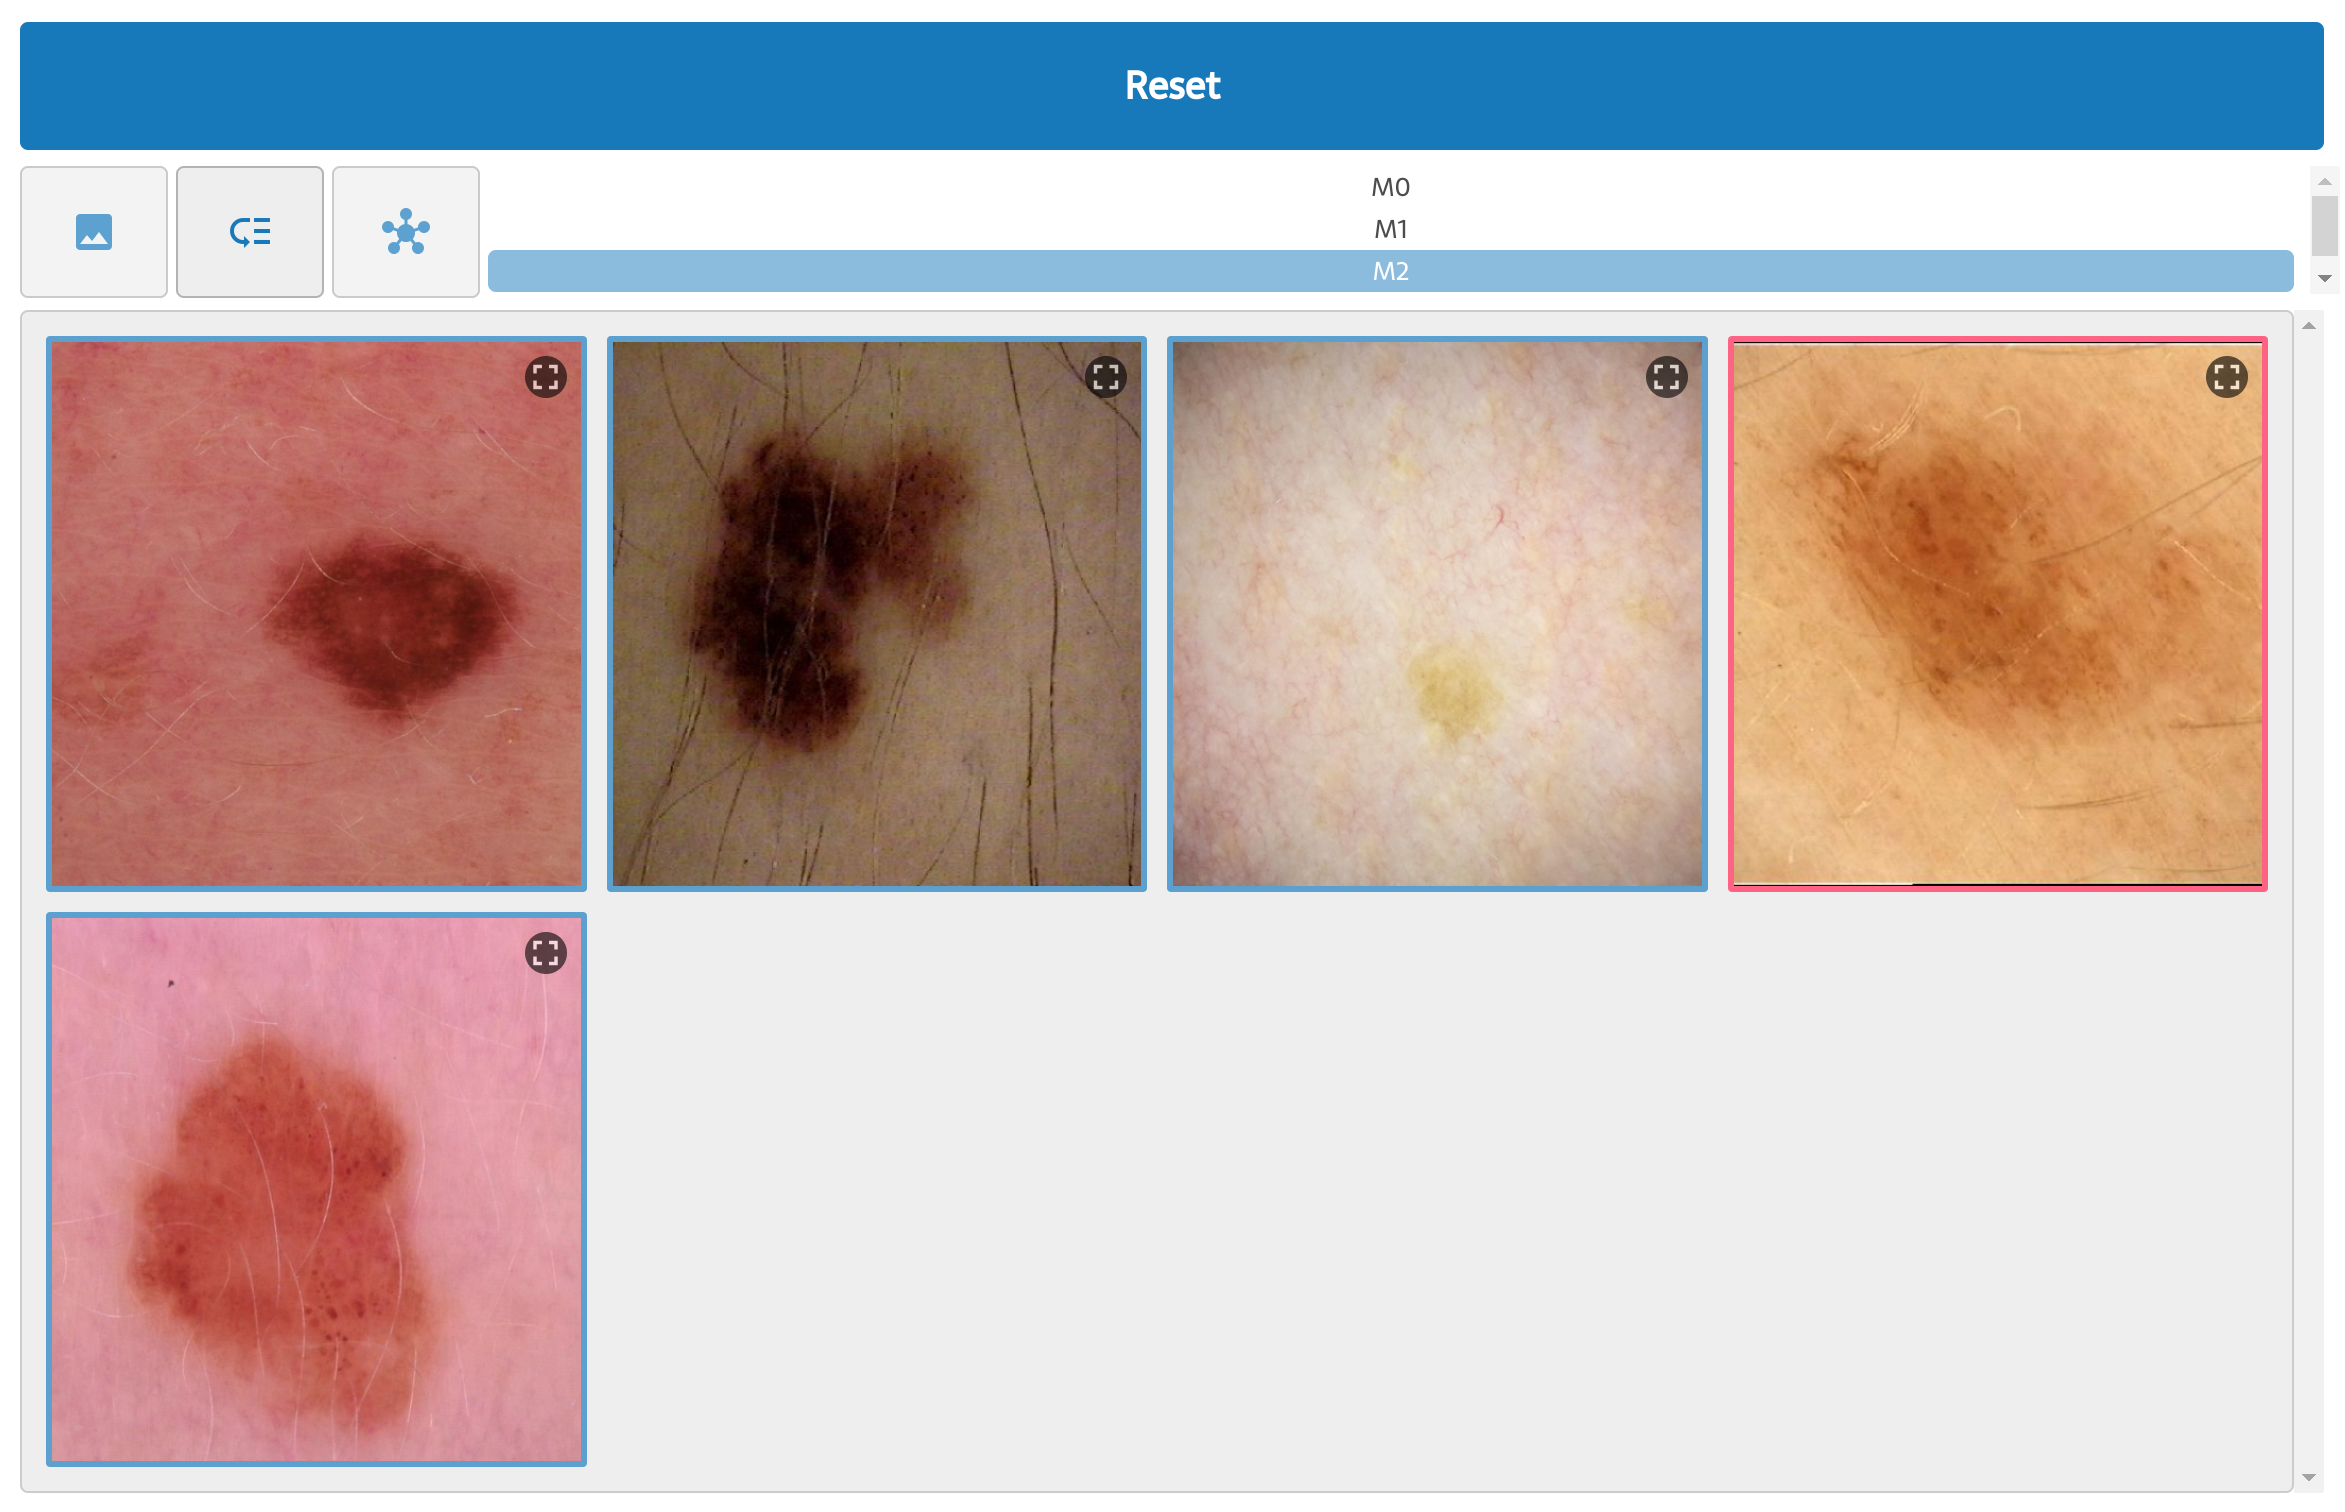
\includegraphics[width=\textwidth]{imatges/results/after-prediction.png}
  \end{adjustbox}
  \caption[UI state after prediction response]{\textit{UI state after prediction response. }}
  {\label{fig:after-prediction}}
\end{figure}


\newpage

\begin{figure}[H]
  \centering
  \begin{adjustbox}{width=\textwidth, trim={0.05cm 0cm 0.25cm 0cm}, clip}
    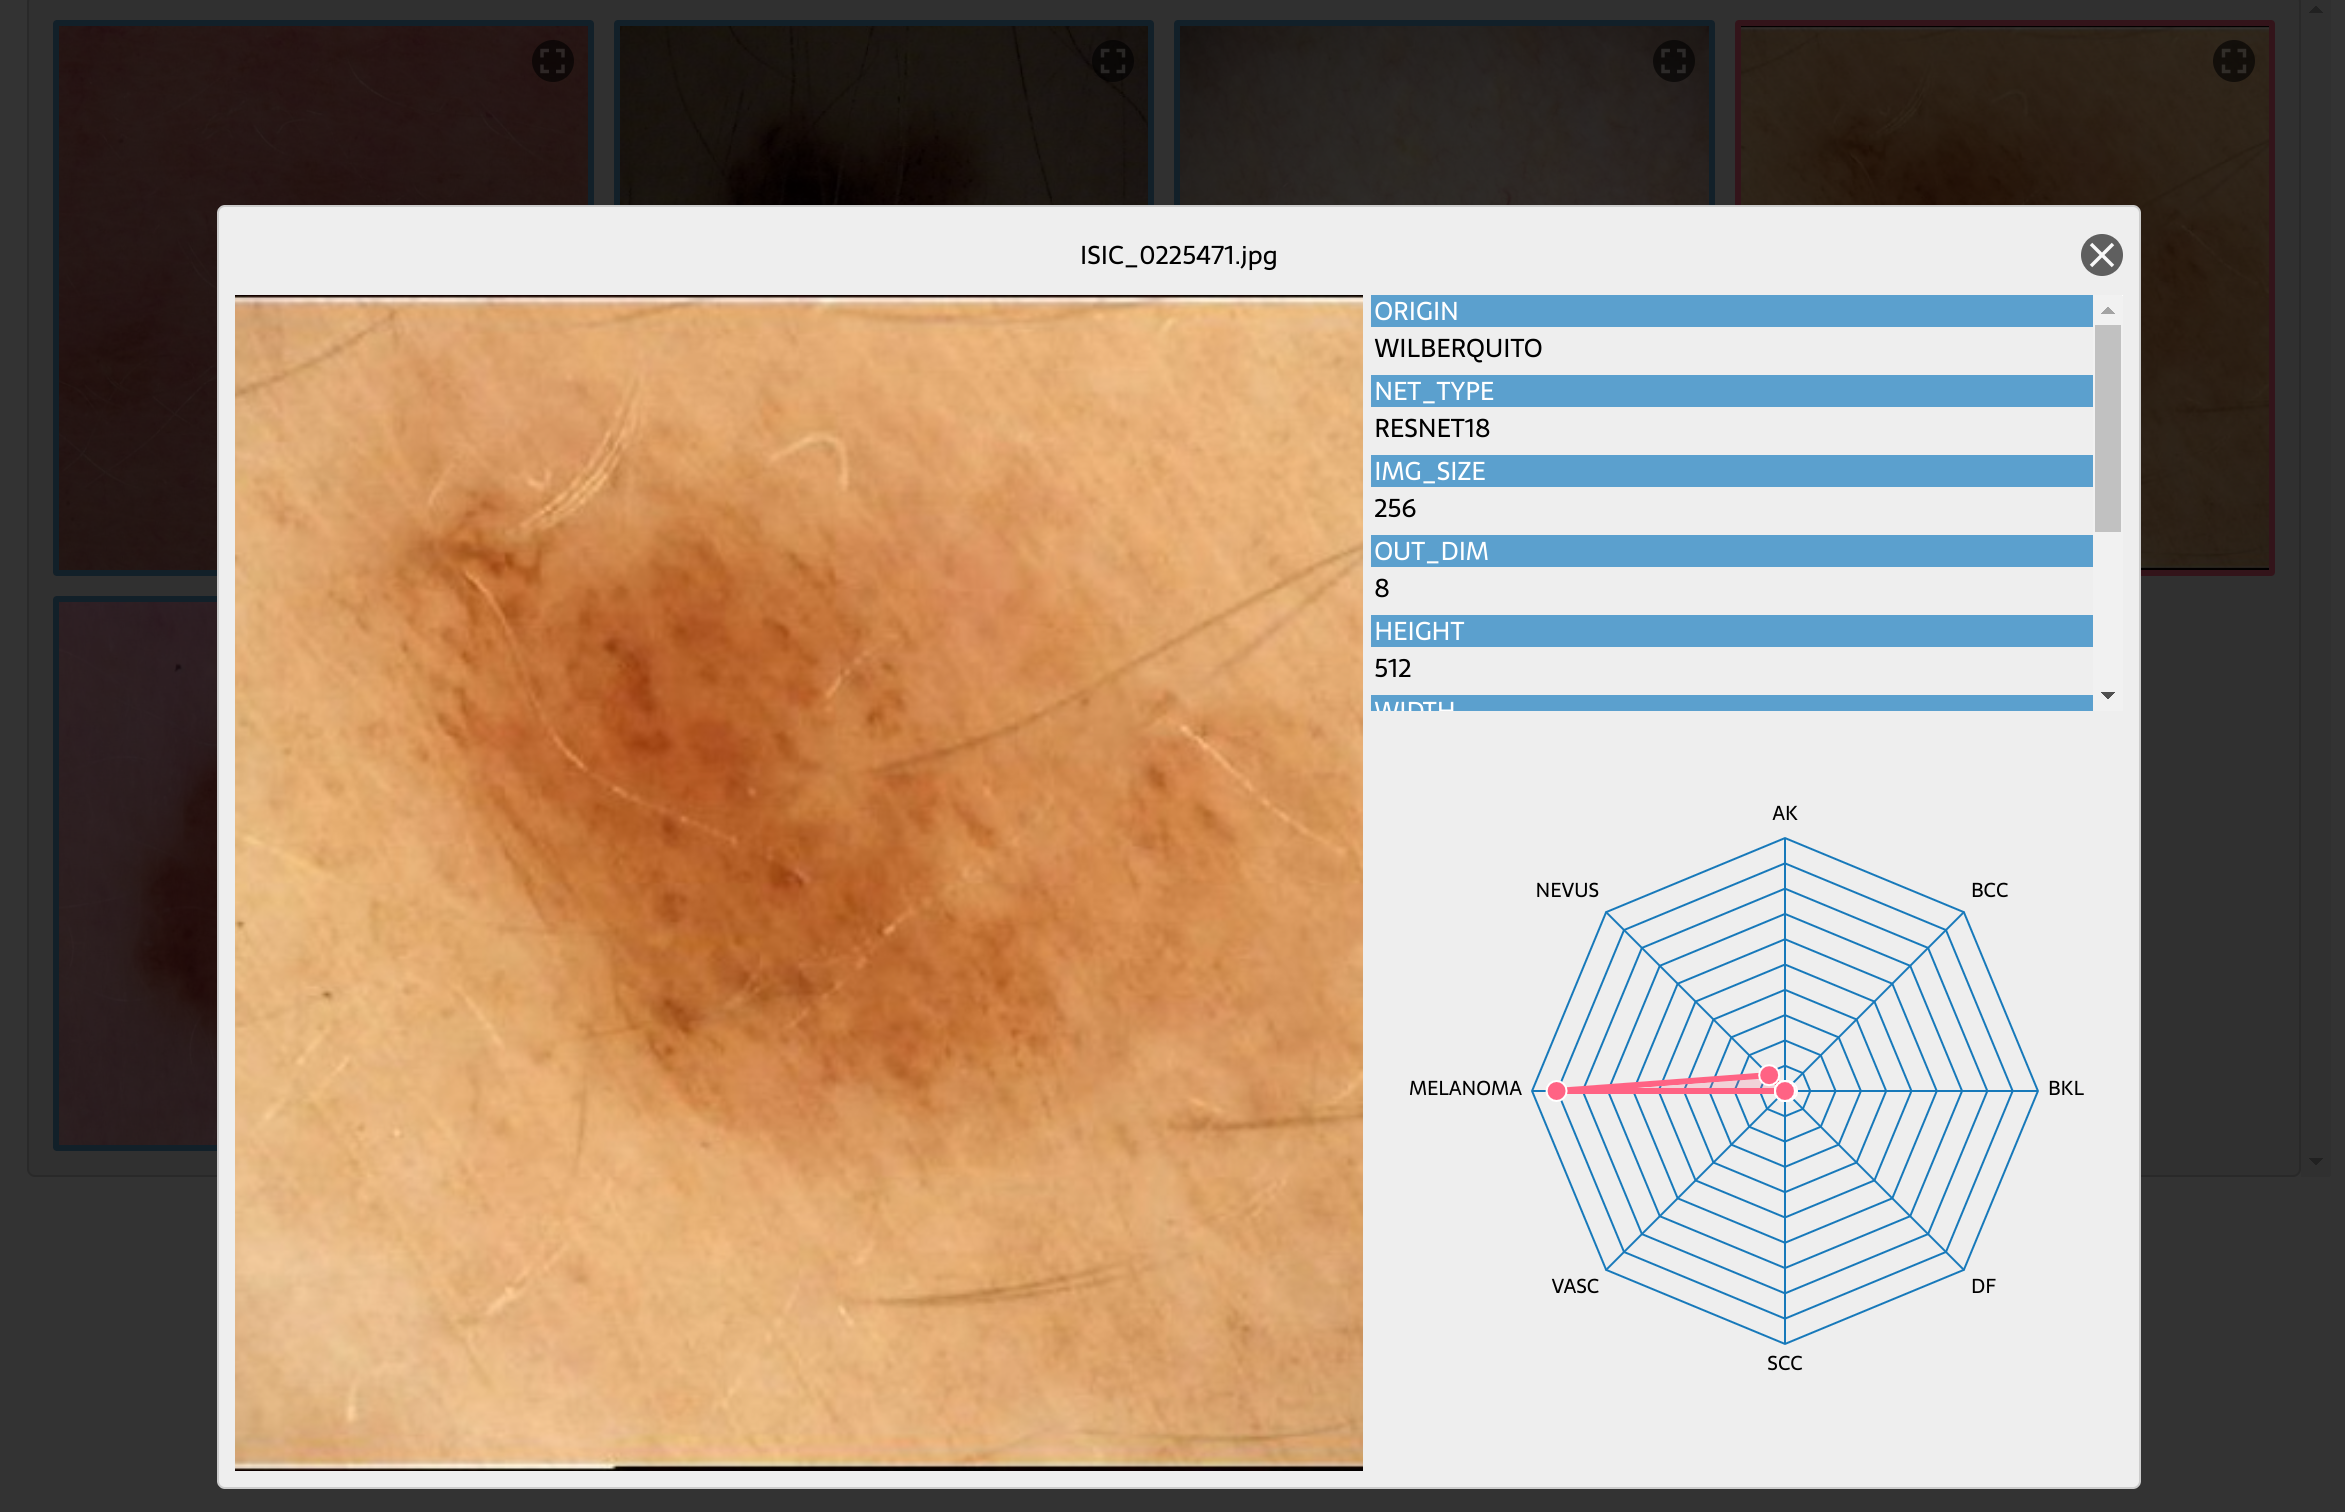
\includegraphics[]{imatges/results/extra-inf-popup.png}
  \end{adjustbox}
  \caption[Extra prediction information]{\textit{Extra prediction information.}}
  {\label{fig:extra-inf-popup}}
\end{figure}

\newpage
